\begin{figure}[h]
	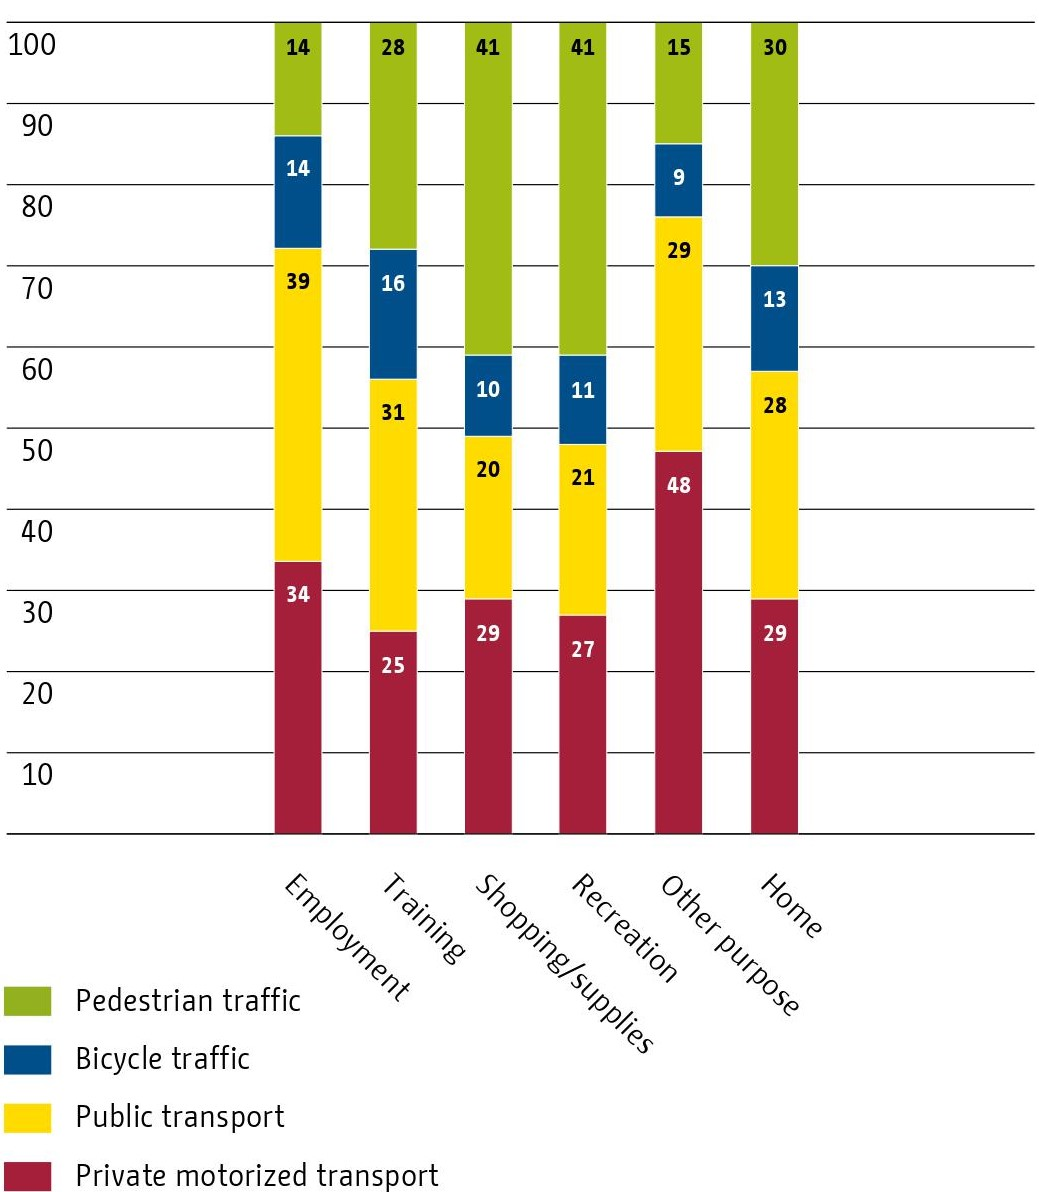
\includegraphics[width=0.5\textwidth]{MobilityInTheCityJPG/Graphs/UseOfTransportPurpose.jpg}
	\centering
	\caption{Use of transport mode by purpose of journey.\cite{MobilityCity}}
\end{figure}
\section{Car}

With a length of approximately 5400 Km of roads the car remains the most used mean of transport for commuting. Improving the roads and making more parking spaces available makes the car an attractive option. However, only 20\% of the road vehicles travelling in Berlin are private cars. The other 80\% cars are vehicles belonging to flexible, non-binding schemes and with a fixed pick-up point.  The main traffic roads\footnote{Main traffic roads: they have a total length of 160 km.} ensures that people coming from Berlin's suburbs or nearby cities reach the minor roads efficiently (Figure \ref{motorways}). The vast majority of these minor roads (370 km) have a speed limit of 30 km/h upon them, which is due to safety reasons and noise control\cite{MobilityCity}. \\ \newline
The demand for parking spaces is significantly higher than the supply, but this is where Berlin's parking policy plays a big role. A 100,000 parking spaces across 45 parking zones provides a reasonable amount of place to store the commuters vehicle during day or night. Nevertheless parking in Berlin can get expensive. If you live in Berlin and you want to park in your neighbourhood you need a permit\footnote{In German: Bewohnerparkausweis} which costs \texteuro20.40 and is valid for two years. Otherwise you have to pay at the parking meter. Outside the \textit{Ringbahn}\footnote{Berliner Ringbahn: a 37.5 km long circle route around Berlin's inner area, on the Berlin S-Bahn network.} you can park for free. Other costs like car insurance (\texteuro100 to \texteuro1000 per year), vehicle tax\footnote{Kraftfahrzeugsteuer} (around \texteuro100 per year), fuel, a vehicle inspections per two years (\texteuro100), maintenance and repairs make the use of the car for commuting an expensive option\cite{CostCars}.

\begin{figure}[h]
	\begin{minipage}[c]{0.4\linewidth}
		\centering
		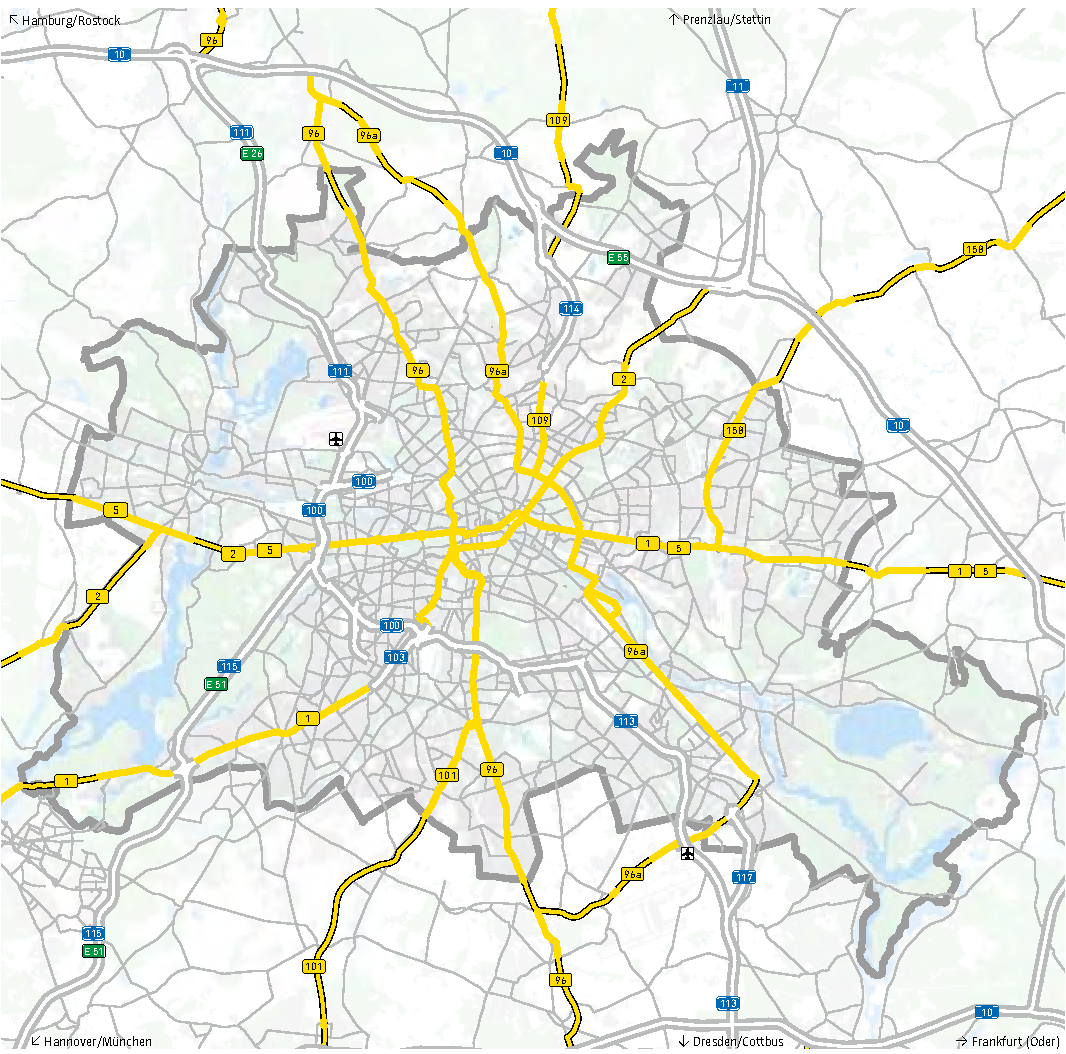
\includegraphics[height=7cm]{MobilityInTheCityJPG/Graphs/Motorways.pdf}
		\caption{Motorway and major road network}
		\label{motorways}
	\end{minipage}\hfill
	\begin{minipage}[c]{0.5\linewidth}
		\centering
		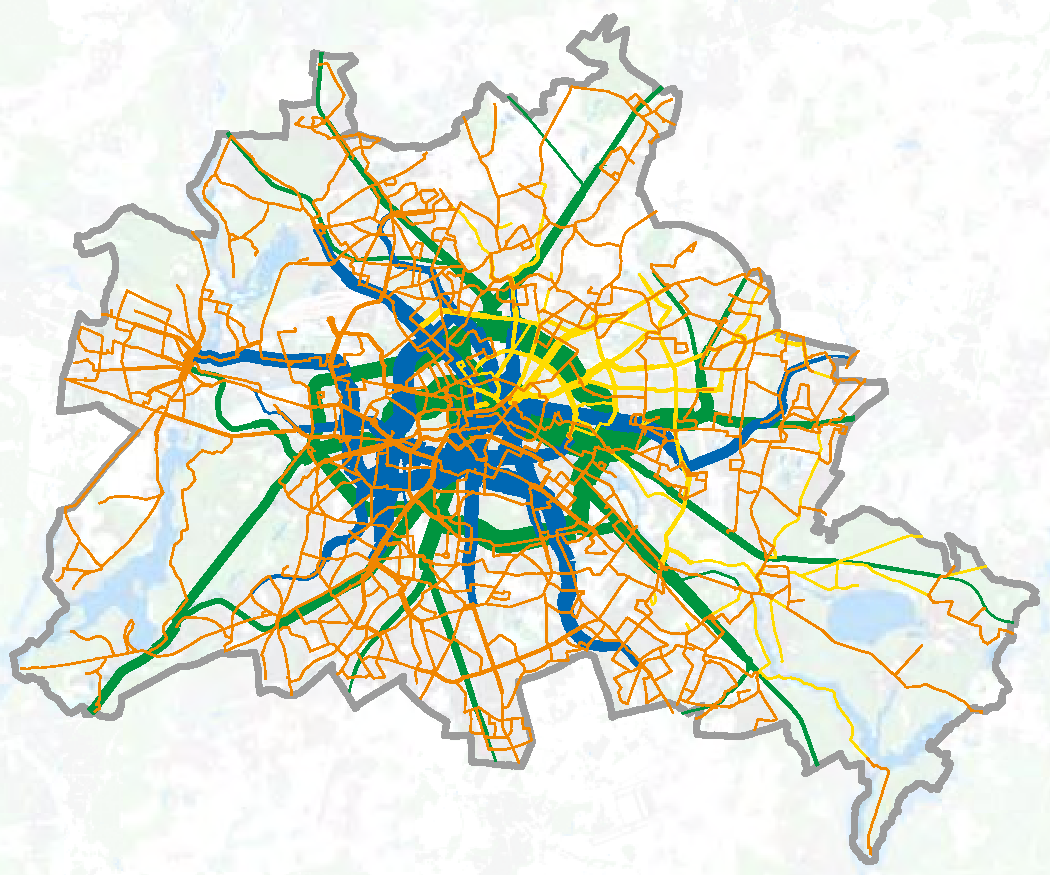
\includegraphics[height=7cm]{MobilityInTheCityJPG/Graphs/PTnetwork.pdf}
		\caption{Public transport network by transport mode}
		\label{ptnetwork}
	\end{minipage}
\end{figure}


\section{Bus}

The bus network consists of a large network that covers almost the entire city of Berlin (orange lines in Figure \ref{ptnetwork}). The network consists of 149 daytime and 63 night bus routes, seventeen MetroBus and 13 express routes.  The day lines connect the suburbs with the central city or S-Bahn and U-Bahn stations. The night bus lines replace partially certain U-Bahn lines and the most important day lines. The MetroBuses give service in areas that are poorly served by the U-Bahn and S-Bahn. They are designated as part of the \textit{MetroNetz} and serve 24 hours per day, seven days per week, in intervals of ten minutes. The X-buses (express) are faster routes which is accomplished through a small number of the more important stops on the route. By the greater distance between the stops, the buses lose less time on stopping the vehicle\cite{xpress}. \\

\subsection*{BVG}
The \textit{Berliner Verkhersbetriebe} (BVG\footnote{BVG: An abbreviation from the original company \textit{\textbf{B}erliner \textbf{V}erkehrs-Aktien\textbf{g}esellschaft}}) is the main public transport company of Berlin. It coordinates and develops the U-Bahn, tram, bus, replacement services and ferry networks\cite{BVG1}. With their 3,000 vehicles, they transported 1,064 million passengers in 2016 or more than 2.7 million passengers per day\cite{MobilityCity}.


\section{Tram}
 The tram network in Berlin was founded in 1865 and is hereby one of the oldest there is. After Melbourne and St. Petersburg, it's the largest tram system in the world. Since 1929, the BVG has operated the system\cite{tram}. By 1967, due to the Cold War and the division of Berlin in East and West Berlin, most tram lines that ran along West Berlin had closed, resulting in only two operational tram lines. The trace of the division is still visible, seeing that most tram lines are still in East Berlin\cite{tramz}. It's made of 22 lines and measuring almost 190 km in route length. Also here there are nine Metrotrams that give service 24 hours per day with small intervals\cite{tram}. 
 
\section{Train}
\subsection{S-Bahn} \label{sebsec:sBahn}

Since 1930, the \textit{Berliner S-Bahn} has been operational in and around Berlin. This rapid transit railway system\footnote{Rapid transit: type of high-capacity public transport generally found in urban areas.} works complementary with the U-Bahn and connects the city centre with the suburbs. Through the high frequency and travel possibilities throughout Berlin and beyond, the S-Bahn has the characteristics of the combination between a commuter rail service and a rapid transit system. This railway system has three characteristics that make this public transportation mode unique. Vehicles that use the term S-bahn, are provided of a third-rail electrical power transmission\footnote{Third rail: A method of providing electric power to a train, through a semi-continuous rigid conductor placed alongside the rails of the track\cite{thirdRail}.}, the Berlin S-Bahn loading gauge\footnote{A loading gauge defines the maximum height and width for railway vehicles and their loads to ensure that they can pass safely through tunnels and under bridges\cite{gauge}.} and a communications-based train control system specific to the S-Bahn, in opposite of the usual automated mechanical train control system. The S-Bahn network consists of 16 lines serving 166 stations and has a total route length of 332 km. Three core lines can be seen when look at the S-Bahn: a central, elevated east-west line, a central, mainly underground north-south line and a circular line. All lines begin to disperse upward of the \textit{S-Bahn Ring}\cite{SBahn}. Per year the S-Bahn transports 334 million passengers and one million commuters per work day\cite{SBahnFIGURES}.\\ \newline
Opposed to trams and buses, which are operated by the BVG, the S-Bahn is part of the \textit{S-Bahn Berlin GmbH}, a company that is completely owned by the \textit{Deutsche Bahn}, a private, joint-stock and German railway company, with the Federal Republic of Germany being its single shareholder\cite{DB}.

\subsection{U-Bahn}

Together with the tram network and the S-Bahn, the U-Bahn is definitely the main means of transport in the German capital. The \textit{Untergrundbahn} opened in 1902 and serves currently 175 metrostations across nine lines, which make a total length of 155 km. The metro vehicles run every five minutes during the day, every ten minutes during the evening and from two to five minutes during peak hours. The U-Bahn is operated by the BVG\cite{UBahn}.

\section{Ticketing system and price}
\begin{figure}[h]
	\begin{minipage}[c]{0.4\linewidth}
		\centering
		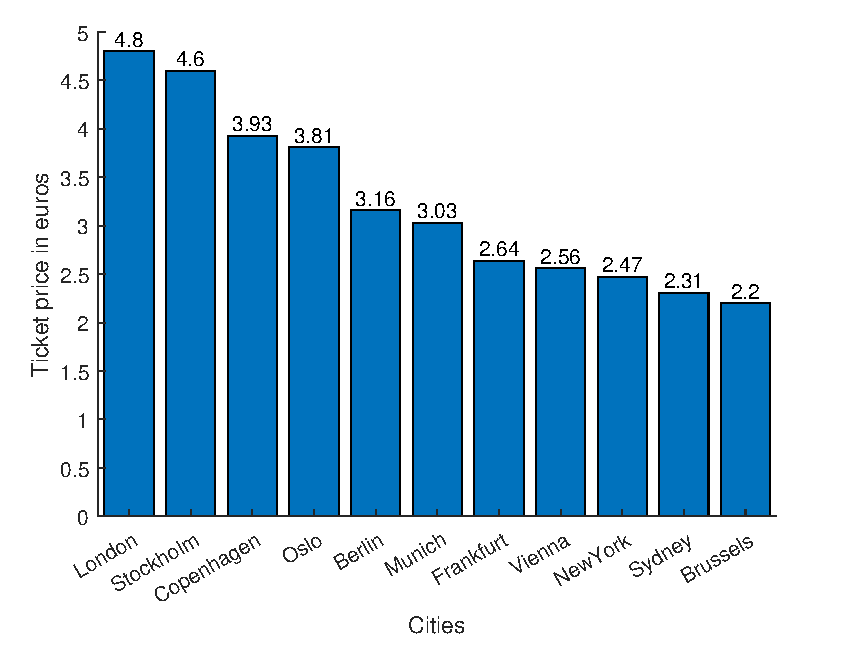
\includegraphics[height=7cm]{Images/GraphPricePT.pdf}
		\caption{Average cost for public transport (bus, tram or metro) in selected cities around the world in 2017\cite{pricesPT}.}
		\label{pricePT}
	\end{minipage}\hfill
	\begin{minipage}[c]{0.45\linewidth}
		\centering
		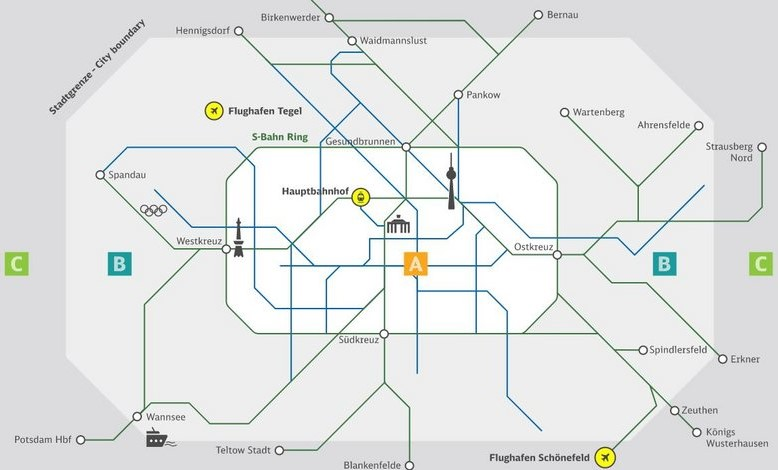
\includegraphics[width=1.1\linewidth]{Images/tariffZones.jpg}
		\caption{Tariff zones of Berlin demarcated according to the S-bahn train lines\cite{tarif}.}
		\label{tariffZones}
	\end{minipage}
\end{figure}
As shown on Figure \ref{tariffZones}, Berlin's divided into three tariff zones A, B and C. Zone A surrounds the city centre and the circular \textit{S-Bahn Ring}, zone B reaches the city limits and zone C includes the suburbs and Potsdam. The latter also belongs to the counties surrounding the city. Depending on the destination tickets can be bought for AB, BC or ABC\cite{tarif}. A normal one way ticket costs respectively \texteuro3.00, \texteuro3.50 or \texteuro3.80. Moreover there are short distance tickets\footnote{Short distance tickets cost \texteuro2.00 and are valid for three stops of the S- and U-Bahn or six stops of buses and trams.}, 24 hour tickets, group tickets ...  Tickets can be bought at ticket machines located at train stations, on buses, in trams, ticket counters in larger stations or the mobile app. Tickets must be validated by stamping them at the means of transport\cite{ticketing1}. \\ \newline
On figure \ref{pricePT} the average cost for public transport in cities around the world is displayed. The data is based on the price of a single ticket in 2017 for public transport for a journey of approximately 10 km or at least 10 stops. The first five cities are indeed the five most expensive countries for using public transport and that includes Berlin, which makes the German capital almost 45\% more overpriced than Brussels.


\section{Bike (sharing system)}

On average, the Berliners make 44 \% of their journey on foot or by bicycle. Plus, since 2001, over 450 new crossing facitities have been constructed on the Berlin roads. and the city has currently well over 1,000 km of cycle paths, which concludes that the mobility in the city certainly is oriented towards the pedestrian and bicycle traffic. The bicycle paths can differ extensively in type: mandatory paths, off-road routes, shared bus lanes open to cyclists ... Additional \textit{Fahrradstrassen} give priority to the cyclists and make the cars slow down to 30 km/h. If a bike ticket is purchased, it's possible to take your bike on the S- and U-Bahn, on trams and on night buses\cite{MobilityCity}\cite{cycling}. \\ \newline
In the beginning of 2018 bike sharing companies were booming immensely, but now a few decent companies survived the hype. Currently there are five active bike sharing companies operating in Berlin. The best known dealers are Nextbike, Call a Bike and Lime bikes. Their prices all lay around the same number: \texteuro1-1.5 for the first 30 minutes and then \texteuro1-1.5 per 30 minutes after that. All three of them do require to drop the bike off whithin the S-Bahn circular ring, so it isn't possible for people who live in the suburbs to take the bike to their front door\cite{bikeshare}.


\section{Sharing systems}

